Which of the following sets are convex?

\begin{enumerate}
\item A \textit{slab}, i.e., a set of the form $\{x \in \mathbb{R}^n \mid \alpha \leq a^T x \leq \beta\}$. \defpoints{4}
\item A \textit{rectangle}, i.e., a set of the form $\{x \in \mathbb{R}^n \mid \alpha_i \leq x_i \leq \beta_i, i = 1, \dots, n\}$. A rectangle is sometimes called a \textit{hyperrectangle} when 			$n > 2$. \defpoints{4}
\item A \textit{wedge}, i.e., $\{x \in \mathbb{R}^n \mid a_1^T x \leq b_1, a_2^T x \leq b_2\}$. \defpoints{4}
\item The set of points closer to a given point than a given set, i.e.,
\[\{x \mid \|x - x_0\|_2 \leq \|x - y\|_2 \ \text{for all} \ y \in S\}\]
where $S \subseteq \mathbb{R}^n$. \defpoints{4}
\item The set of points closer to one set than another, i.e.,
\[\{x \mid \text{dist}(x, S) \leq \text{dist}(x, T)\},\]
where $S, T \subseteq \mathbb{R}^n$, and
\[\text{dist}(x, S) = \inf \{\|x - z\|_2 \mid z \in S\}.\] \defpoints{4}
\end{enumerate}

\textcolor{blue}{Solution}
\begin{itemize}
\item[1.] Let $C_1=\{x \in \mathbb{R}^n \mid (-a)^T x \leq -\alpha\}$, and $C_2=\{x \in \mathbb{R}^n \mid a^T x \leq \beta\}$.

$C_1$ and $C_2$ are two halp-spaces, which are convex sets. \\
And since the intersection of two convex sets is also a convex set.

So $C=C_1\cap C_2=\{x \in \mathbb{R}^n \mid \alpha \leq a^T x \leq \beta\}$ is a convex set.

So the slab is a convex set.


\item[2.] Let $C=\{x \in \mathbb{R}^n \mid \alpha_i \leq x_i \leq \beta_i, i = 1, \dots, n\}$.

$\forall x,y\in C,\theta\in[0,1]$, we have $\forall i=1,\dots,n, \alpha_i\leq x_i,y_i\leq\beta_i$.

Let $z=\theta x+(1-\theta)y$, then $\forall i=1,\dots,n$, we have:
\begin{align*}
z_i &= \theta x_i + (1-\theta)y_i \geq \theta\alpha_i + (1-\theta)\alpha_i = \alpha_i \\
z_i &= \theta x_i + (1-\theta)y_i \leq \theta\beta_i + (1-\theta)\beta_i = \beta_i
\end{align*}
i.e. $\alpha_i \leq z_i \leq \beta_i, \forall i=1,\ldots,n$, so $z\in C$.

So $C$ is a convex set.


\item[3.] Let $C_1=\{x \in \mathbb{R}^n \mid a_1^T x \leq b_1\}$, and $C_2=\{x \in \mathbb{R}^n \mid a_2^T x \leq b_2\}$. So $C_1, C_2$ are two half-spaces, which are convex sets. \\
And since the intersection of two convex sets is also a convex set.

So $C=C_1\cap C_2=\{x \in \mathbb{R}^n \mid a_1^T x \leq b_1, a_2^T x \leq b_2\}$ is a convex set.

So the wedge is a convex set.


\item[4.] Let $C=\Big\{x~\vert~\|x-x_0\|_2\leq\|x-y\|_2~\text{for all}~y\in S\Big\}$.\\
$\forall x\in C$, and for a fixed $y$, we have
\begin{align*}
    \|x-x_0\|_2 &\leq \|x-y\|_2 \\
    \|x-x_0\|_2^2 &\leq \|x-y\|_2^2 \\
    (x-x_0)^T(x-x_0) &\leq (x-y)^T(x-y)\\
    (y-x_0)^Tx &\leq \dfrac{1}{2}\left(\|y\|_2^2-\|x_0\|_2^2\right)
\end{align*}

From the definition, we know that for a fixed $y$,
$(y-x_0)^Tx \leq \dfrac{1}{2}\left(\|y\|_2^2-\|x_0\|_2^2\right)$ is a half-space $S_{y}$.

So $\forall y\in S$, we could see that $C=\bigcap\limits_{y\in S}S_{y}$.\\
And since each $S_{y}$ is a half-space, which is a convex set. And from the theorem we have known, that
the intersection of convex sets is also a convex set, so $C$ is a convex set.

\item[5.] $C=\{x \mid \text{dist}(x, S) \leq \text{dist}(x, T)\}$ is not convex. \\
We can construct a counter-example: \\
Let $n=2$, and $S=\left\{(2,2),(-2,-2)\right\}\subseteq\mathbb{R}^2$, $T=\left\{(2,-2),(-2,2)\right\}\subseteq\mathbb{R}^2$, as it's shown above.

\begin{figure}[htbp]
    \centering
    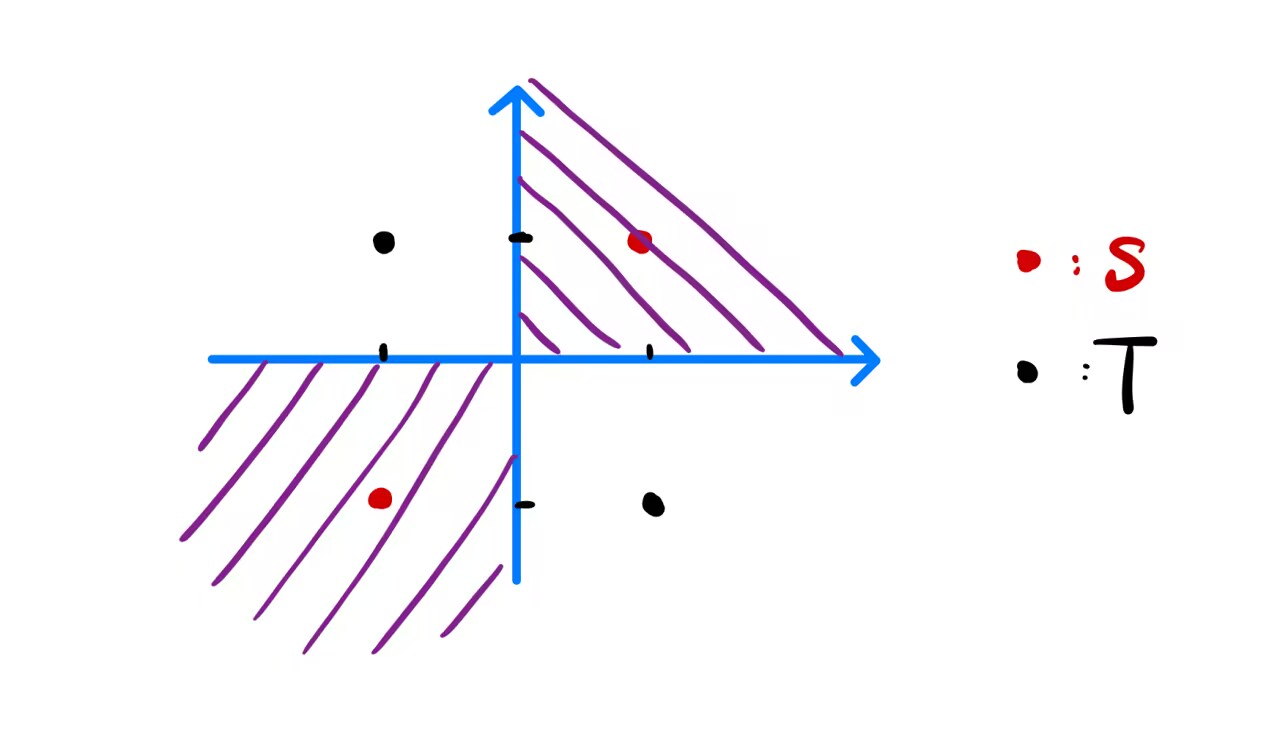
\includegraphics[width=0.6\textwidth]{../counter_example.png}
\end{figure}

And it is clear that $C=\{x \mid \text{dist}(x, S) \leq \text{dist}(x, T)\}=\{(x,y)\mid (x\geq 0\land y\geq 0)\lor(x\leq 0\land y\leq 0)\}$, which is not a convex set.

For example, we have $(x_1,y_1)=(2,0)\in C, (x_2,y_2)=(0,-2)\in C, \theta=\dfrac{1}{2}\in[0,1]$, \\ but $\theta(x_1,y_1)+(1-\theta)(x_2,y_2)=(1,-1)\notin C$.

So we have constructed a counter-example to show that $C$ is not a convex set.

\end{itemize}

\newpage
